%\documentclass[prb,11pt,tightenlines,twocolumn,aps]{revtex4-1}
\documentclass[floatfix,prb,aps,superscriptaddress,showpacs,11pt,preprint,letterpaper]{revtex4}
\usepackage{amsmath}    % need for subequations 
\usepackage{graphicx}   % need for figures 
\usepackage{verbatim}   % useful for program listings 
\usepackage{color}      % use if color is used in text 
\usepackage{subfigure}  % use for side-by-side figures 
\usepackage{hyperref}   % use for hypertext links, including those to external 
                        % documents and URLs 
\usepackage[dvipsnames]{xcolor}
\usepackage{multirow}
%\usepackage[inline]{showlabels}
\input{/Users/bms/util/definitions}
\def\tama{10cm}
\raggedbottom           % don't add extra vertical space

\begin{document}

\title{Pure Spin Current Injection in Hydrogenated Graphene Structures}
\author{Reinaldo Zapata-Pe\~na}
\affiliation{Centro de Investigaciones en \'Optica, Le\'on,
Guanajuato 37150, M\'exico}
\author{Bernardo S. Mendoza}
\affiliation{Centro de Investigaciones en \'Optica, Le\'on,
Guanajuato 37150, M\'exico}
\author{Anatoli I. Shkrebtii}
\affiliation{University of Ontario, Institute of Technology,
Oshawa, ON, L1H 7L7, Canada}

\date{\today}

\begin{abstract}
We present a theoretical study of spin-velocity injection of a pure
spin current induced by  a linearly
polarized beam of light that impinges normally on the surface of  two 50\%
hydrogenated noncentrosymmetric 2D graphene 
structures, labeled Up and Alt.
The hydrogenation opens an energy gap in both structures.
We analyze two possibilities: one in which by fixing the spin along a
chosen direction, the resulting spin-velocity is calculated, 
and another where we choose the spin-velocity direction
on the surface plane, and calculate its speed and
spin orientation. We do so by changing the energy $\hbar\go$ 
and polarization angle $\ga$  of the incoming  beam. 
The results are calculated within a full
electronic band structure scheme within the DFT in the LDA approximation.
The maxima of the spin-velocity speed are obtained when
$\hbar\go=0.084$\,eV and $\ga=35^\circ$ for Up,
and
$\hbar\go=0.720$\,eV and $\ga=150^\circ$ for Alt.
We find a speed of
668\,Km/s
and 
645\,Km/s
for Up and Alt, respectively, when the spin points perpendicularly to
the surface. Also,
the response is maximized
by fixing the spin-velocity direction along a high symmetry Cartesian axis,
obtaining a speed of 
688\,Km/s 
with the spin  pointing at 13$^\circ$ from the surface normal, for Up,
and
906\,Km/s 
and the spin pointing at 60$^\circ$ from the surface normal, for Alt.
These speed values are larger than those of bulk semiconductors, like
CdSe and GaAs, thus 
making the hydrogenated graphene structures
 excellent candidates for spintronics
applications.
\end{abstract}

\maketitle

%%%%%%%%%%%%%%%%%%%%%%%%%%%%%%%%%%%%%%%%%%%%%%%%%%%%%%%%%%%%%%%%%%%%%%%%%%%%%%
%%%%%%%%%%%%%%%%%%%%%%%%%%%%%%%%%%%%%%%%%%%%%%%%%%%%%%%%%%%%%%%%%%%%%%%%%%%%%%
%%%%%%%%%%%%%%%%%%%%%%%%%%                         %%%%%%%%%%%%%%%%%%%%%%%%%%%
%%%%%%%%%%%%%%%%%%%%%%%%%% I N T R O D U C T I O N %%%%%%%%%%%%%%%%%%%%%%%%%%%
%%%%%%%%%%%%%%%%%%%%%%%%%%                         %%%%%%%%%%%%%%%%%%%%%%%%%%%
%%%%%%%%%%%%%%%%%%%%%%%%%%%%%%%%%%%%%%%%%%%%%%%%%%%%%%%%%%%%%%%%%%%%%%%%%%%%%%
%%%%%%%%%%%%%%%%%%%%%%%%%%%%%%%%%%%%%%%%%%%%%%%%%%%%%%%%%%%%%%%%%%%%%%%%%%%%%%

\section{Introduction}
\label{sec:introduction}


Spintronics is an emerging research field of electronics in which the
manipulation and transport of spin of electrons in a solid state 
media plays the determining role, adding a new degree of freedom to
conventional charge manipulation.\cite{wolfSC04,fabianAPS07}
% 
At present, there is an increasing interest in attaining the same level of
control over the transport of spin at micro or nano scales, as it has been done for
the flow of charge in typical electronic devices.\cite{awschalomNP2007} Some
semiconductor spintronics devices have been proposed \cite{majumdarAPL06,
dattaAPL90,gotteNat16,pershinPRB08}, and some of them require spin polarized
electrical current \cite{awschalomSSBM13} or pure spin current (PSC).
% 
One of the difficulties to achieve the development of spin current and PSC
semiconductor devices is the fact that the spin relaxation time in a
semiconducting media is short, disabling the spin transport, and then resulting
in a non-observable spin current.\cite{murakamiSc03}
% 
In PSCs, there is no net
motion of charge; spin-up electrons move in a given direction, while spin-down
electrons travel in the opposite one. 
This effect can result from one photon absorption of linearly polarized light
by a semiconductor, with filled valence bands and empty conduction bands,
illuminated by light with photon energy larger than the energy gap.
This phenomenon can result from spin
injection,\cite{malPRB03} Hall Effects,\cite{sinovaPRB04} interference of two
optical beams,\cite{bhatPRL00, najmaiePRB03} or one photon absorption of
linearly polarized light\cite{bhatPRL05} and has been observed in gallium
arsenide (GaAs),\cite{zhaoPRL2006, stevensPRL03} aluminum-gallium arsenide
(AlGaAs),\cite{stevensPRL03} and Co$_2$FeSi.\cite{kimuraNGPAM12}

Graphene, an allotrope of carbon with hexagonal 2D lattice structure, presents
properties like fractional quantum Hall effect at room temperature, excellent
thermal transport properties, excellent conductivity\cite{heerscheNat07} and
strength \cite{geimNM07, reinaNL08, novoselov2S07, balandinNL08}, being then a
perfect platform to be used in two-dimension electronic systems; however, most
electronic applications are disabled by the absence of a semiconducting gap.
Recent studies demonstrate that the band gap of graphene can be opened by
applying an electric field,\cite{zhangN09} reducing the surface
area,\cite{hanPRL07} or applying uniaxial strain.\cite{niACSN08} Another
possibility to open the gap is by doping; this has been successfully achieved
using nitrogen,\cite{weiNL2009} boron-nitrogen,\cite{guoIJ11}
silicon,\cite{colettiPRB10} noble-metals,\cite{varykhalovPRB10} and
hydrogen.\cite{eliasS09, guisingerNL09, samarakoonACSN10}
% 
Depending on the percentage of hydrogenation and spatial configurations of
hydrogen-carbon bonds, hydrogenated graphene can result in different spatial
configurations.
% 
In this paper, we present two 50\% hydrogenated graphene noncentrosymmetric
structures, both presenting a discernible band gap: the Up structure,
shown in Fig. \ref{fig:up-struc}, has hydrogen atoms bonded to the carbon layer
only on the upper side of the structure, while the Alt structure, shown
in Fig. \ref{fig:alt-struc}, has hydrogen alternating on the upper and bottom
sides of the carbon slab.\cite{zapataPSB2016}

\begin{figure}[ht!]
    \centering
    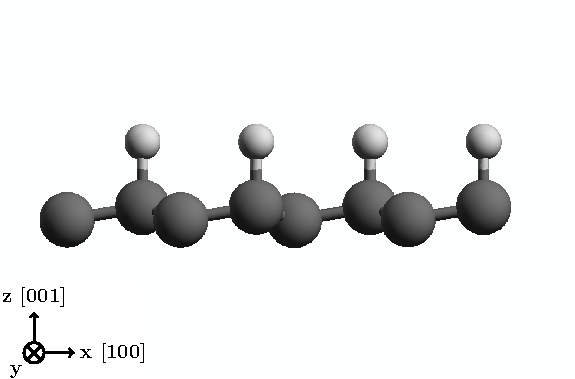
\includegraphics[width=\tama]{figures/upstruc2}
    \\
    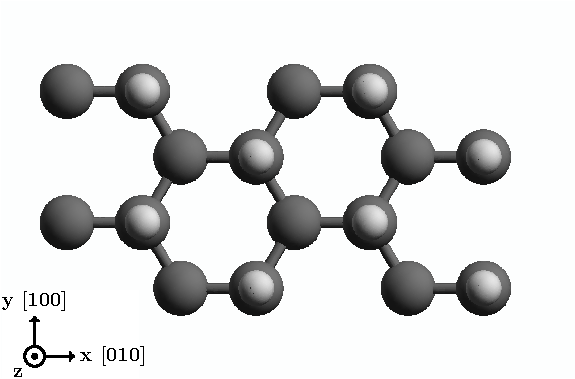
\includegraphics[width=\tama]{figures/upstruc1}
    \caption{Side (top panel) and top (bottom panel) views of the Up
      structure along with the 
      Cartesian $xyz$ directions. The dark (light) spheres are the C (H) atoms,
      labeled 1 (2).
}
    \label{fig:up-struc}
\end{figure}
\begin{figure}[ht!]
    \centering
    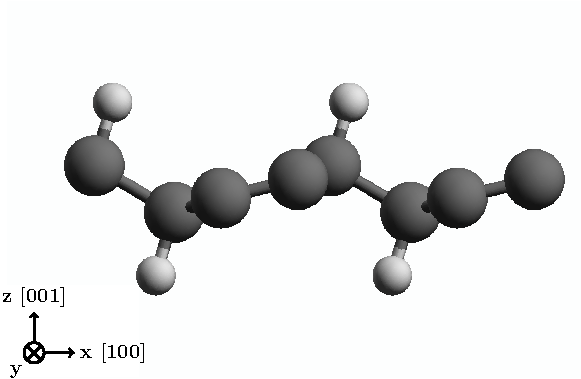
\includegraphics[width=\tama]{figures/altstruc2}
    \\
    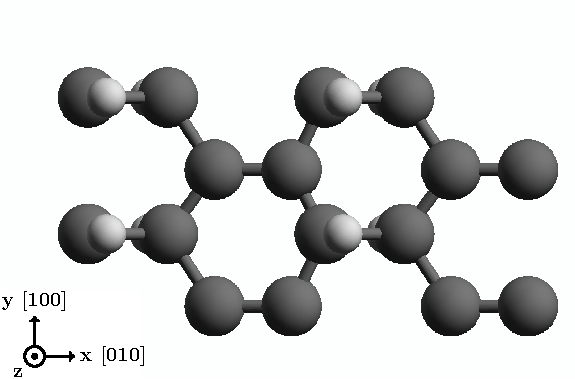
\includegraphics[width=\tama]{figures/altstruc1}
    \caption{Side (top panel) and top (bottom panel) views of the Alt
      structure along with the 
      Cartesian $xyz$ directions. The dark (light) spheres are the C (H) atoms,
      labeled 1 (2).
}
    \label{fig:alt-struc}
\end{figure}


Using those structures, we address a theoretical study of the 
spin velocity
injection (SVI) 
by one-photon absorption of linearly polarized light.
Since we have 2D structures, we do the analysis for two cases. The first is by
fixing the spin of the electrons along the $z$ Cartesian direction, with the
velocity directed on the surface of the structure on the $xy$ plane. The second
is by fixing the spin velocity in the $x$ or $y$ direction and the spin directed
to $xyz$.
% 
The SVI is an optical effect that quantifies the velocity at which a PSC moves
along the Cartesian direction, $\mathrm{a}$, with the spin of electron polarized
along the Cartesian direction $\mathrm{b}$. One photon absorption of linearly
polarized light can promote an even distribution of electrons in $\mathbf{k}$ space,
regardless of the symmetry of the material, resulting in a 
null electrical current.\cite{bhatPRL05}
Then, the electrons excited to the conduction bands at opposite $\mathbf{k}$
points will result in opposite spin polarizations producing no net spin
injection.\cite{bhatPRL05} If the crystalline structure of the material is
noncentrosymmetric, the spin polarization injected at a given $\mathbf{k}$ point
not necessarily 
 vanishes,\cite{alvaradoPRL85, schmiedeskampPRL88} 
and then, since the velocities of electrons at opposite $\mathbf{k}$ points are
opposite, a PSC will be produced. Since the structures presented
here are noncentrosymmetric, they are good candidates in which this effect can
be induced.

This paper is organized as follows. In Section \ref{sec:theory} we present the
theory and formulas that describe PSC and SVI. In Section \ref{sec:results} we
describe the details of calculations and the corresponding SVI spectra for the
Up and Alt structures. Finally, we present our conclusions in
Section \ref{sec:conclusions}.


%%%%%%%%%%%%%%%%%%%%%%%%%%%%%%%%%%%%%%%%%%%%%%%%%%%%%%%%%%%%%%%%%%%%%%%%%%%%%%
%%%%%%%%%%%%%%%%%%%%%%%%%%%%%%%%%%%%%%%%%%%%%%%%%%%%%%%%%%%%%%%%%%%%%%%%%%%%%%
%%%%%%%%%%%%%%%%%%%%%%%%%%%%%%%%               %%%%%%%%%%%%%%%%%%%%%%%%%%%%%%%
%%%%%%%%%%%%%%%%%%%%%%%%%%%%%%%%  T H E O R Y  %%%%%%%%%%%%%%%%%%%%%%%%%%%%%%%
%%%%%%%%%%%%%%%%%%%%%%%%%%%%%%%%               %%%%%%%%%%%%%%%%%%%%%%%%%%%%%%%
%%%%%%%%%%%%%%%%%%%%%%%%%%%%%%%%%%%%%%%%%%%%%%%%%%%%%%%%%%%%%%%%%%%%%%%%%%%%%%
%%%%%%%%%%%%%%%%%%%%%%%%%%%%%%%%%%%%%%%%%%%%%%%%%%%%%%%%%%%%%%%%%%%%%%%%%%%%%%

\section{Theory} % (fold)
\label{sec:theory}


%%%%%%%%%%%%%%%%%%%%%%%%%%%%%%%%%%%%%%%%%%%%%%%%%%%%%%%%%%%%%%%%%%%%%%%%%%%%%%
%%%%%%%%%%%%%%%%%%%%%%%%%%% Theory: Spin velocity %%%%%%%%%%%%%%%%%%%%%%%%%%%%
%%%%%%%%%%%%%%%%%%%%%%%%%%%%%%%%%%%%%%%%%%%%%%%%%%%%%%%%%%%%%%%%%%%%%%%%%%%%%%


In this section, we report a summary of the theory  involved in the
calculation of the spin velocity
injection (SVI) resulting from the
pure spin current (PSC).
 
%%%BMSD
The operator that describes the electronic SVI is written as
\begin{align}\label{z.1}
\hat K^{\rma\rmb}=\frac{1}{2}\left( \hat v^\rma \hat S^\rmb 
+\hat  S^\rmb \hat v^\rma\right) 
,
\end{align} 
where $\hat\bfv=[\hat\bfr,\hat H_0]/i\hbar$ is the velocity operator, with
$\hat \bfr$ being the position operator and $\hat H_0$ the unperturbed
ground state Hamiltonian;
the Roman superscripts  indicate Cartesian coordinates. 
To obtain the expectation value of 
$\hat K^{\rma\rmb}$, we use the length gauge for the perturbing
Hamiltonian, written as
\begin{align}\label{z.2}
\hat H_{\text{p}}=-e\hat\bfr\cdot\bfE(t)
,
\end{align}   
where the electric field of the applied laser is given by
\begin{align}\label{z.3}
\bfE(t)= \bfE(\go)e^{-i\go t} + \bfE^*(\go)e^{i\go t}
.
\end{align}
In order to 
calculate the response of the system to $\bfE(t)$, one needs to
take into account the excited coherent superposition
of the spin-split conduction bands inherent to the 
noncentrosymmetric 
semiconductors considered in this work.
%Although, this splitting is small [15,16], is required to obtain the
%correct results\cite{nastosPRB07}.
% The conduction bands in the 
% noncentrosymmetric  
% semiconductors  
% are spin split by a small amount,[15,16] typically
%   smaller than the energy width of the laser pulse, and so the pulse
%   excites a coherent superposition of the two conduction bands. Even
%   for very long pulses with narrow energy widths, dephasing effects
%   lead to an energy width of the bands large enough that spin-split
%   states can become quasidegenerate. 
To include the coherences, we follow Ref.~\onlinecite{nastosPRB05} and
use a multiple
scale approach that solves the equation of motion for the single
particle density matrix $\gr_{mn}(\bfk;t)$, leading to
\begin{align}\label{z.4}
&\frac{\partial \rho_{cc'}(\bfk)}{\partial t} =
\frac{e^{2}E^{\mathrm{a}}(\omega)E^{\mathrm{b*}}(\omega)}
{i \hbar^{2}}
\sum_{v}r^{\mathrm{a}}_{cv}(\bfk) r^{\mathrm{b}}_{vc'}(\bfk)
\left( \frac{1}{\omega - \omega_{c'v}(\bfk) - i \epsilon} 
- 
\frac{1}{\omega - \omega_{cv}(\bfk) + i \epsilon} \right)
,
\end{align}
where we assumed that the conduction bands $c$ and $c'$
are quasidegenerate  states, and we take $\ge\to 0$ at the end of the
calculation.  The spin-splitting of the valence ($v$) bands is very
small, and is neglected throughout this work.\cite{nastosPRB07}
% 􏱈 are close to  
% one another, and that the pulse is short enough so that the energy
% width overlaps the two bands, the equation of motion can be
% solved. Leaving the details of the derivation to Ap- 
% pendix A, the result for the off-diagonal component 􏰠 􏱈, c  
%%%BMSU 
The matrix elements of any operator $\calo$ are given by
$\calo_{nm}(\bfk)=\bra{n\bfk}\hat\calo\ket{m\bfk}$,
where 
$H_{0}|n\mathbf{k}\rangle = \hbar \omega_{n}(\mathbf{k})|n\mathbf{k}\rangle$ 
with $\hbar \omega_{n}(\mathbf{k})$ being the energy of the
electronic band $n$ at point $\mathbf{k}$ in the irreducible Brillouin zone
(IBZ),  $|n\mathbf{k}\rangle$ is the Bloch state, and 
$\go_{nm}(\bfk)=\go_{n}(\bfk)-\go_{m}(\bfk)$.
Using 
$\mathcal{O} = \mathrm{Tr}(\hat{\rho}\hat{\mathcal{O}})$
for the expectation value of an observable $\mathcal{O}$, 
where $\mathrm{Tr}$ denotes the trace, we obtain
\begin{align}\label{z.5}
\mathcal{O} 
%=&
%\int \frac{d^{3}k}{8\pi^{3}}\sum_{c} \langle c \mathbf{k} 
%| \hat{\rho} \hat{\mathcal{O}} |
%c\mathbf{k} \rangle \nonumber \\
=& 
\int \frac{d^{3}k}{8\pi^{3}} \sum_{cc'} \rho_{cc'}(\mathbf{k}) 
\mathcal{O}_{c'c}(\mathbf{k}),
\end{align}
where we used 
the closure
relationship $\sum_{n}|n\mathbf{k}\rangle \langle n\mathbf{k}| = 1$,
where $n=v,c$,
and the fact that $\rho_{vn}(\bfk)=\rho_{nv}(\bfk)=0$ for $n=c,c'$. 
Therefore, 
using  Eqs. \eqref{z.4} and \eqref{z.5},
the
rate of change of $\mathcal{O}$,
$\dot{\mathcal{O}} 
=
\mathrm{Tr} \left( \dot{\hat\rho} \hat\calo \right)
$,
 is given by
\begin{align}
\dot{\mathcal{O}} 
&=\frac{e^{2}}{i\hbar^{2}} \int \frac{d^{3}k}{8\pi^{3}} 
\sum'_{cc'} \mathcal{O}_{c'c}(\bfk) 
r^{\mathrm{a}}_{cv}(\bfk)  r^{\mathrm{b}}_{vc'}(\bfk)  
\left( \frac{1}{\omega - \omega_{c'v}(\bfk)  - i\epsilon} - 
\frac{1}{\omega - \omega_{cv}(\bfk)  + i\epsilon} \right)
E^{\mathrm{a}}(\omega) E^{\mathrm{b*}}(\omega)
\label{eq:dotO}
.
\end{align}
Replacing  $\hat\calo \rightarrow \hat{K}^{\mathrm{ab}}$, in 
the above expression, one can show that
\begin{equation}
\dot{K}^{\mathrm{ab}}(\omega) =
\mu^{\mathrm{abcd}}(\omega)
E^{\mathrm{c}}(\omega) E^{\mathrm{d*}}(\omega),
\label{eq:dotk}
\end{equation}
where repeated Cartesians are summed, and 
\begin{equation}\label{eq:mu}
\begin{aligned}
\mu^{\mathrm{abcd}}  (\omega) &
=
\frac{\pi e^{2}}{\hbar^{2}} \int 
\frac{d^{3}k}{8 \pi^{3}} \sum'_{vcc'}
  \delta(\omega-\omega_{cv}(\bfk) 
\mathrm{Re} & \left[ K^{\mathrm{ab}}_{cc'}(\bfk) 
\left(  
r^{\mathrm{c}}_{vc'}(\bfk)   
r^{\mathrm{d}}_{cv }(\bfk)  +
(c \leftrightarrow d)  
\right) 
\right]
\end{aligned}
\end{equation} 
is the pseudotensor that describes the rate of change of the  PSC process in
semiconductors. To derive above we used
$
K^{\mathrm{ab}}_{nm}(\mathbf{-k}) = K^{\mathrm{ab*}}_{nm}(\mathbf{k}) 
$
which follows from time-reversal invariance. The prime symbol $'$ in the sum means that
$c$ and $c'$ are quasi degenerate states, and the sum only covers these states.
Since $\mu^{\mathrm{abcd}}(\omega)$ is real, we have that
$\mu^{\mathrm{abcd}}(\omega) =
\mu^{\mathrm{abdc}}(\omega)$. 
We remark that Eq.~\eqref{eq:mu} 
is the same as Eq. (3) of Bhat et al.\cite{bhatPRL05},
obtained by using the semiconductor optical Bloch equations.
Using the closure relation,
\begin{equation}
K^{\mathrm{ab}}_{cc'}(\mathbf{k}) = \frac{1}{2}
\sum_{l=v,c}
\left(v^{\mathrm{a}}_{cl}(\mathbf{k})S^{\mathrm{b}}_{lc'}(\mathbf{k})
+S^{\mathrm{b}}_{cl}(\mathbf{k}) v^{\mathrm{a}}_{lc'}(\mathbf{k})
\right)
.
\label{eq:velspimatelem}
\end{equation}

%%%%%%%%%%%%%%%%%%%%%%%%%%%%%%%%%%%%%%%%%%%%%%%%%%%%%%%%%%%%%%%%%%%%%%%%%%%%%%
%%%%%%%%%%%%%%%%%%%%%%%%%%%%%%%%%%%%%%%%%%%%%%%%%%%%%%%%%%%%%%%%%%%%%%%%%%%%%%

%\subsection{Spin velocity injection} % (fold)
%\label{sec:theory-pure_spin_current}
Now, we define the spin velocity injection (SVI) as
\begin{equation}\label{eq:vab-w}
\mathcal{V}^{\mathrm{ab}}(\omega) \equiv
\frac{\dot{K}^{\mathrm{ab}}(\omega)}{(\hbar/2) \dot{n}(\omega)},
\end{equation}  
which gives the velocity, along direction $\mathrm{a}$, at which the spin
moves in a polarized state along direction $\mathrm{b}$. The carrier injection rate
$\dot n(\go)$ is written as,\cite{nastosPRB05}
\begin{equation}
\dot{n}(\omega) =
\xi^{\mathrm{ab}}(\omega) E^{c }(\omega) E^{d*}(\omega)
\label{eq:dotn}
\end{equation}
where the tensor 
\begin{equation}\label{eq:xi}
\begin{aligned}
\xi^{\mathrm{ab}}(\omega)
&
=
\frac{2\pi e^{2}}{\hbar^{2}} \int 
\frac{d^{3}k}{8 \pi^{3}}
 \sum_{vc}
r^{\mathrm{a}}_{vc'}(\bfk)  
r^{\mathrm{b}}_{cv }(\bfk)  
\delta(\omega-\omega_{cv}(\bfk) 
, 
\end{aligned}
\end{equation}
is related to the imaginary part of the linear optical 
response tensor by
$\mathrm{Im}[\ge^{\rma\rmb}(\go)]=2\pi\ge_0\hbar\xi^{\rma\rmb}(\go)$.

The function $\calv^{\rma\rmb}(\go)$ allows us to quantify two very
important aspects of PSC. On one hand, we can fix the spin direction
along $\mathrm{b}$  
and calculate the resulting electron velocity.  
On the other hand, we can fix the velocity of the electron
along $\mathrm{b}$ and study the resulting direction along which the
spin is polarized.
To this end, the added advantage of  2D structures, besides choosing
them as noncentrosymmetric, is that we can use an incoming linearly
polarized beam of light
at normal incidence, and use the  direction of the polarized  electric
field to control $\calv^{\rma\rmb}(\go)$.
Indeed, writing 
$\bfE(\omega) = E_0(\omega)(\cos\ga\,\hat\bfx+\sin\ga\,\hat\bfy)$,
where $\alpha$ is the polarization angle, we obtain from
 Eq. \eqref{eq:vab-w}
that
\begin{widetext}
\begin{align}
\mathcal{V}^{\mathrm{ab}}(\omega,\alpha)
&= 
\frac{2}{\hbar\xi(\go)}
\left(\mu^{\mathrm{abxx}}(\omega)\cos^{2}\alpha + 
\mu^{\mathrm{abyy}}(\omega)\sin^{2}\alpha + 
\mu^{\mathrm{abxy}}(\omega)\sin 2\alpha\right)
,
\label{eq:vab-aw}
\end{align}
\end{widetext}
for the structures chosen in this article,
$\xi^{\mathrm{xx}}(\go)=\xi^{\mathrm{yy}}(\go)\equiv\xi(\go)$, and $\xi^{\mathrm{xy}}(\go)=0$.
Now, we formalize our two options for $\calv^{\rma\rmb}(\go)$.

\subsection{Fixing spin}\label{sec:theory-fixspin}

Analyzing the SVI, Eq. \eqref{eq:vab-aw}, we define the magnitude of
the electron velocity on the plane of the structure 
with the spin polarized along the $\mathrm{b}$ direction as
\begin{equation}
\mathcal{V}_{\sigma^{\mathrm{b}}}(\omega,\alpha)
\equiv
\sqrt{
[\mathcal{V}^{\mathrm{xb}}(\omega,\alpha)]^{2}\ +
[\mathcal{V}^{\mathrm{yb}}(\omega,\alpha)]^{2}\ 
}, 
\label{eq:vs-mag}
\end{equation}
and define the angle at which the velocity is directed on the $xy$ plane as
\begin{equation}
\gamma_{\gs^\mathrm{b}} (\omega,\alpha)
=
\tan^{-1} \left( \frac{\mathcal{V}^{\mathrm{yb}}(\omega,\alpha)}
{\mathcal{V}^{\mathrm{xb}}(\omega,\alpha)} \right)
.
\label{eq:gamma-ang}
\end{equation}
% where this angle is measured in the counter-clockwise direction from the
% positive $x$. 
We also define two special angles
\begin{equation}
\gamma_{\gs^\mathrm{b}}^\parallel(\omega,\alpha) = \alpha, 
\label{eq:gamma-par} 
\end{equation}
and
\begin{equation}
\gamma_{\gs^\mathrm{b}}^\perp(\omega,\alpha) = \alpha \pm 90^{\circ},
\label{eq:gamma-perp}
\end{equation}
corresponding to the electron velocity being parallel or perpendicular
to the incoming polarization, 
respectively. The subscript $\gs^\rmb$ denotes the spin along $\rmb$.

%%%%%%%%%%%%%%%%%%%%%%%%%%%%%%%%%%%%%%%%%%%%%%%%%%%%%%%%%%%%%%%%%%%%%%%%%%%%%%
%%%%%%%%%%%%%%%%%%%%%%%%%%%% Theory: Fixing vel %%%%%%%%%%%%%%%%%%%%%%%%%%%%%%
%%%%%%%%%%%%%%%%%%%%%%%%%%%%%%%%%%%%%%%%%%%%%%%%%%%%%%%%%%%%%%%%%%%%%%%%%%%%%%


\subsection{Fixing velocity.}\label{sec:theory-fixvel}

Fixing the calculated velocity along $\rma=x$ or $\rma=y$,
we define its corresponding magnitude as
\begin{align}
\mathcal{V}_{\mathrm{a}}(\omega,\alpha) \equiv 
\sqrt { 
[\mathcal{V}^{\mathrm{ax}}(\omega,\alpha)]^{2} +
[\mathcal{V}^{\mathrm{ay}}(\omega,\alpha)]^{2} +
[\mathcal{V}^{\mathrm{az}}(\omega,\alpha)]^{2} 
},
\label{eq:vv-mag}
\end{align}
from where we see that the spin would be oriented
in the $xyz$ system's coordinates
according to a polar angle
\begin{align}
\theta_{\mathrm{a}}  (\omega,\alpha)
= 
\cos^{-1} \left( \frac{\mathcal{V}^{\mathrm{az}}(\omega,\alpha)}
{\mathcal{V}_{\mathrm{a}}(\omega,\alpha)} \right),
 \quad 0 \leq \theta \leq \pi, 
\label{eq:polar-ang}
\end{align}
and an azimuthal angle
\begin{align}
\varphi_{\mathrm{a}} (\omega,\alpha)
=
\tan^{-1} \left( \frac{\mathcal{V}^{\mathrm{ay}}(\omega,\alpha)}
{\mathcal{V}^{\mathrm{ax}}(\omega,\alpha)} \right),
\quad 0 \leq \varphi \leq 2\pi.
\label{eq:azimuthal-ang} 
\end{align} 


%%%%%%%%%%%%%%%%%%%%%%%%%%%%%%%%%%%%%%%%%%%%%%%%%%%%%%%%%%%%%%%%%%%%%%%%%%%%%%
%%%%%%%%%%%%%%%%%%%%%%%%%%%%%%%%%%%%%%%%%%%%%%%%%%%%%%%%%%%%%%%%%%%%%%%%%%%%%%
%%%%%%%%%%%%%%%%%%%%%%%%%%%%%                   %%%%%%%%%%%%%%%%%%%%%%%%%%%%%%
%%%%%%%%%%%%%%%%%%%%%%%%%%%%%   R E S U L T S   %%%%%%%%%%%%%%%%%%%%%%%%%%%%%%
%%%%%%%%%%%%%%%%%%%%%%%%%%%%%                   %%%%%%%%%%%%%%%%%%%%%%%%%%%%%%
%%%%%%%%%%%%%%%%%%%%%%%%%%%%%%%%%%%%%%%%%%%%%%%%%%%%%%%%%%%%%%%%%%%%%%%%%%%%%%
%%%%%%%%%%%%%%%%%%%%%%%%%%%%%%%%%%%%%%%%%%%%%%%%%%%%%%%%%%%%%%%%%%%%%%%%%%%%%%

\section{Results} % (fold)
\label{sec:results}

\begin{table}[t]
\center
\begin{tabular}{ccccc}\\
\hline
\quad Layer \quad & \quad Atom \qquad & \multicolumn{3}{c}{Position (\AA)} \\
\cline{3-5}
\quad No.   \quad & \quad type \qquad & $x$ & $y$ & $z$  \\
\hline
1 & H & -0.61516 & -1.77416 &  0.73196 \\
1 & H &  0.61518 &  0.35514 &  0.73175 \\
2 & C & -0.61516 & -1.77264 & -0.49138 \\
2 & C & -0.61516 & -0.35600 & -0.72316 \\
2 & C &  0.61516 &  0.35763 & -0.49087 \\
\hline
\end{tabular}

\caption{Unit cell of Up structure. Layer division, atom types and
positions for the Up structure. The structure unit cell was divided in
two layers corresponding to hydrogen and carbon atoms.The corresponding layer
atom position is depicted in Fig. \ref{fig:up-struc} with the corresponding
number of layer.}
\label{tab:up-unitcell}
\end{table}
% 
% 
\begin{table}[t]
\center
\begin{tabular}{ccccc}\\
\hline
\quad Layer \quad & \quad Atom \qquad & \multicolumn{3}{c}{Position (\AA)} \\
\cline{3-5}
\quad No.   \quad & \quad type \qquad & $x$ & $y$ & $z$  \\
\hline
1 & H &  -0.61516 &  -1.42140 & \ 1.47237 \\
2 & C &  -0.61516 &  -1.73300 & \ 0.39631 \\
3 & C & \ 0.61516 & \ 1.73300 & \ 0.15807 \\
4 & C & \ 0.61516 & \ 0.42201 &  -0.15814 \\
5 & C &  -0.61516 &  -0.37396 &  -0.39632 \\
6 & H &  -0.61516 &  -0.68566 &  -1.47237 \\
\hline
\end{tabular}

\caption{Unit cell of Alt structure. Layer division, atom types and
positions for the Alt structure. The structure unit cell was divided in
six layers corresponding each one to atoms in different $z$ positions. The
corresponding layer atom position is depicted in Fig. \ref{fig:alt-struc} with
the corresponding number of layer.}
\label{tab:alt-unitcell}
\end{table}

We present the results of $\mathcal{V}_{\sigma^{\mathrm{b}}}(\omega,\alpha)$ and
$\mathcal{V}_{\mathrm{a}}(\omega,\alpha)$ for the C$_{16}$H$_{8}$-up  and
C$_{16}$H$_{8}$-alt structures, being both noncentrosymmetric semi-infinite 2D
carbon systems with 50\% hydrogenation in different arrangements. We recall
that the Up structure has hydrogen atoms only on the upper side of the carbon
sheet, while the Alt structure has alternating hydrogen atoms on the upper and
bottom sides. Also, we take the hexagonal carbon lattice to be on the $xy$ plane
for both structures, and the carbon-hydrogen bonds on the perpendicular $xz$
plane, as depicted in Figs. \ref{fig:up-struc} and \ref{fig:alt-struc}. The
coordinates for the Up and Alt unit cells of the structures are presented in
Tables \ref{tab:up-unitcell} and \ref{tab:alt-unitcell}.

We calculated the self-consistent ground state and the Kohn-Sham states using
density functional theory in the local density approximation (DFT-LDA), with a
planewave basis using the ABINIT code \cite{gonzeCPC09}.
% 
We used Hartwigsen-Goedecker-Hutter (HGH) relativistic separable dual-space
Gaussian pseudopotentials \cite{hartwigsenPRB98}, including the spin-orbit
interaction needed to calculate $\mu^{\mathrm{abcd}}(\omega,\alpha)$ presented
in Eq. \eqref{eq:mu}.
% 
The convergence parameters for the calculations of our results corresponding to
the Up and Alt structures are cutoff energies of 40\,Ha and 65\,Ha, resulting
in LDA energy band gaps of 0.084\,eV and 0.718\,eV, respectively. The energy
eigenvalues and matrix elements for the Up and Alt structures were calculated
using 12802 $\mathbf{k}$ points and 14452 $\mathbf{k}$ points in the IBZ to
integrate $\mu^{\mathrm{abcd}}(\go)$ and $\xi^{\rma\rmb}(\go)$ using the
linearized analytic tetrahedron method (LATM).\cite{nastosPRB07} We neglect the
anomalous velocity term $\hbar(\bfgs\times\nabla V)/4m^2c^2$, where $V$ is the
crystal potential, in $\hat\bfv$ of Eq.~\eqref{z.1}, as this term is known to
give small contribution to PSC.\cite{bhatPRL05} Therefore,
$[\hat\bfv,\hat\bfS]=0$, and Eq.~\eqref{z.1} reduces to $\hat K^{\rma\rmb}=\hat
v^\rma \hat S^\rmb=\hat S^\rmb \hat v^\rma$. Finally, the prime in the sum of
Eq.~\eqref{eq:mu} is restricted to quasidegenerated conduction bands $c$ and
$c'$ that are closer than 30 meV, where this value is both a typical laser-
pulse energy width and the room-temperature energy.\cite{nastosPRB07}
% 
% It is known that the DFT with LDA approximation misestimates the energy band
% gap of semiconductors. To correct this one has to include the many-body
% interaction using i.e. the so-called GW approximation but this technique has a
% very high computational cost and is out of the scope in this paper.
% Nevertheless, DFT still remains a mainstream tool for calculating diverse
% properties derived from the electronic band structure.

%%%%%%%%%%%%%%%%%%%%%%%%%%%%%%%%%%%%%%%%%%%%%%%%%%%%%%%%%%%%%%%%%%%%%%%%%%%%%%
%%%%%%%%%%%%%%%%%%%%%%%%%%% Results: Spin velocity %%%%%%%%%%%%%%%%%%%%%%%%%%%
%%%%%%%%%%%%%%%%%%%%%%%%%%%%%%%%%%%%%%%%%%%%%%%%%%%%%%%%%%%%%%%%%%%%%%%%%%%%%%

\subsection{SVI: Spin velocity injection} % (fold)
\label{sec:res-spin_velocity}

%%%%%%%%%%%%%%%%%%%%%%%%%%%%%%%%%%%%%%%%%%%%%%%%%%%%%%%%%%%%%%%%%%%%%%%%%%%%%%
%%%%%%%%%%%%%%%%%%%%%%%%%% Res: mu & V^{ab} comparison %%%%%%%%%%%%%%%%%%%%%%%
\begin{figure}[t]
\centering
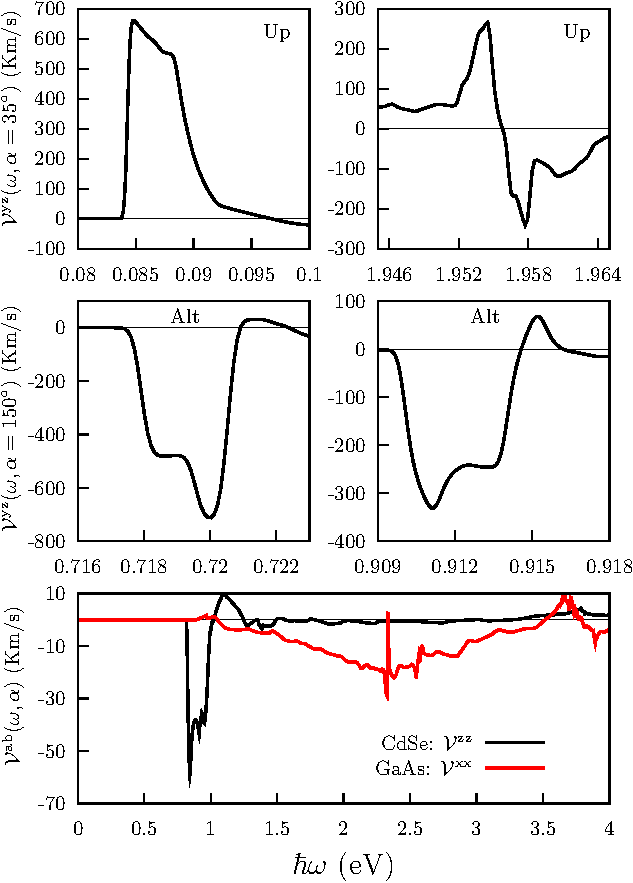
\includegraphics[width=\tama]{plots/2-vab-str-comp}
\caption{$\mathcal{V}^{\mathrm{ab}}(\go,\ga)$ 
  vs. $\hbar\go$, for the values of $\ga$ that maximize the signal. The low
  energy regions for the Alt and Up structures start at the energy gap of each
  structure, while in the high energy regions, the values of
  $\mathcal{V}^{\mathrm{ab}}(\go,\ga)$ are also very large. The bottom panel
  corresponds to CdSe and GaAs. }
\label{fig:vab-str-comp}
\end{figure}

In Fig. \ref{fig:vab-str-comp}, we show $\mathcal{V}^{\mathrm{ab}}
(\omega,\alpha)$ vs. $\hbar\go$ for the directions $\rma\rmb$ and the angle $\ga$
that maximizes the signal, for the Up  and Alt structures and for CdSe and
GaAs, which are bulk systems shown for comparison.
% 
As expected from the delta function of Eq.~\eqref{eq:mu},
$\calv^{\rma\rmb}(\go,\ga)$ rises right at the corresponding energy gap of each
system. For the 2D structures, the spectrum covers two narrow energy regions
with large values of response, while for bulk systems, the spectra covers a
rather wide energy range, but with a much smaller response.
% 
For the Up structure, $\rma\rmb=yz$ and $\ga=35^\circ$ maximize the response,
which means that an incoming beam of light with its electric field polarized at
35$^\circ$ from the $x$ direction will induce electrons to move along $y$
(parallel to the surface), with their spin polarized along $z$ (perpendicular to
the surface), with the following speeds:
% 
right at the energy onset, $\calv^{yz}(\go,\ga)=668$\,Km/s, a speed that remains
almost constant for 65 meV, and then goes to zero and a second region is found
above 1.946 eV, where there are two extreme values of the speed,
$\calv^{yz}(\go,\ga)=266.3$ Km/s at $\hbar\go=1.954$\,eV, and
$\calv^{\rma\rmb}(\go,\ga)=-241.4$ Km/s at $\hbar\go=1.958$\,eV; a positive
(negative) $\calv^{\rma\rmb}(\go,\ga)$ means that the electrons move parallel
(antiparallel) to the electric field.
Likewise, for the Alt structure, we find that also $\rma\rmb=yz$ and
$\ga=150^\circ$ maximizes the response, where two extreme values of
$\calv^{\rmy\rmz}$ are found, one at  $\hbar\go=0.720$\,eV of
$\calv^{\rmy\rmz}=-711.9$ Km/s, and the other at $\hbar\go=0.911$\,eV of
$\calv^{\rmy\rmz}=-330.6$ Km/s.
 
For the bulk structures, we calculate $\calv^{\rma\rmb}(\go)$ from
Eq.~\eqref{eq:vab-w} by simply using $\bfgmu_{\mathrm{max}}$. For CdSe, we find
that for $\hbar\go=0.844$\,eV, $\bfgmu_{\mathrm{max}}\to \mu^{zzzz}$, and
$\calv^{\rmz\rmz}(\go)=-59.0$ Km/s, and for GaAs at $\hbar\go=2.324$\,eV,
$\bfgmu_{\mathrm{max}}\to\mu^{\mathrm{aaaa}}$ and $\calv^{\rma\rma}(\go,\ga)=-28.7$\,Km/s, with
$\rma=x,y,z$. For these bulk semiconductors, the $x$, $y$, and $z$ axis are
taken along the standard cubic unit cell directions, [100], [010], and [001],
respectively. In Table \ref{tab:vab-str-comp}, we present the comparison of
$\calv^{\rma\rmb}(\go,\ga)$ for the 2D structures and bulk crystals.
% 
We remark that, as shown in the figure, 
the 2D structures have maxima in 
$\calv^{\rma\rmb}(\go;\ga)$  
that are bigger
than for the bulk crystals; in particular, the Alt
structure gives a $\calv^{\rma\rmb}(\go;\ga)$ $\sim$12 times larger than
that of CdSe and GaAs.
\begin{table}%[b]
\begin{tabular}{cccccc}
\hline
\multirow{2}{*}{Structure \quad} & 
Kind of \quad & 
Pol. &
Energy & 
\multicolumn{2}{c}{$\mathcal{V}^{\mathrm{ab}}(\omega,\alpha)$}\\
\cline{5-6}
& system & Ang. & [eV] & $\mathrm{ab}$ \quad & [Km/s]\\
\hline
Up    & 2D   & 35    & 0.084  & $\mathrm{yz}$ &  660.5 \\
      &      &       & 1.954  & $\mathrm{yz}$ &  266.3 \\
      &      &       & 1.958  & $\mathrm{yz}$ & -241.4 \\
Alt   & 2D   & 150   & 0.720  & $\mathrm{yz}$ & -711.9 \\
      &      &       & 0.911  & $\mathrm{yz}$ & -330.6 \\
CdSe  & bulk & --    & 0.844  & $\mathrm{zz}$ &  -59.0 \\
GaAs  & bulk & --    & 2.324  & $\mathrm{xx}$ &  -28.7 \\
\hline
\end{tabular}
\caption{Comparison of the reported maximum values of
$\mathcal{V}^{\mathrm{ab}}(\go,\ga)$ for the different structures and their
corresponding polarization angle $\alpha$ and $\hbar\go$ energy values.
}
\label{tab:vab-str-comp}
\end{table}



\subsection{Fixing spin} % (fold)
\label{sec:res-fixspin}

\begin{figure}[t]
\centering
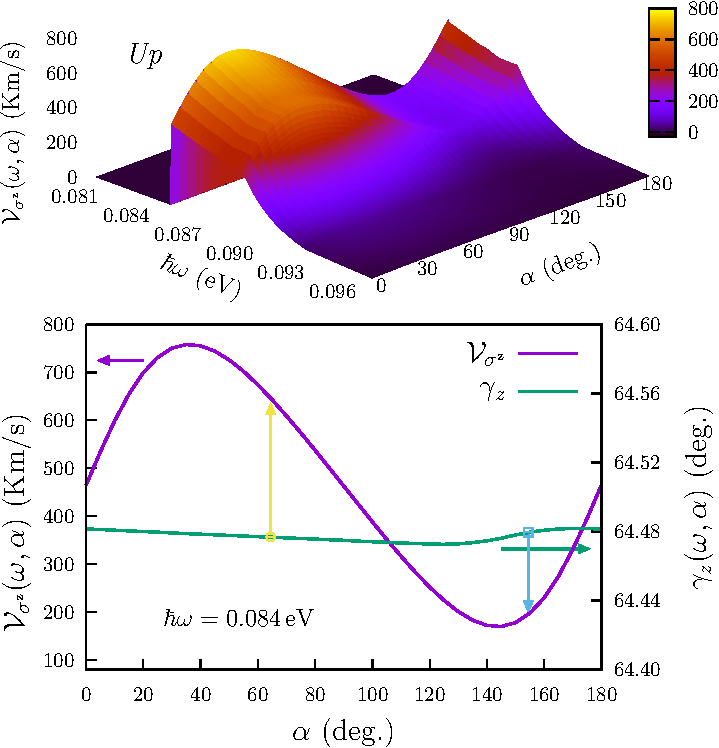
\includegraphics[width=\tama]{upplots/up-vsz-w1}
\caption{For the Up structure, the top panel shows 
$\calv_{\gs^\rmz}(\go,\ga)$ vs. $\hbar\go$ and $\ga$, and the bottom panel
shows $\gamma_{\gs^\rmz}(\go,\ga)$ (right scale, red line), and
$\calv_{\gs^\rmz}(\go,\ga)$ (left scale, black line), vs. $\ga$, for
$\hbar\go=0.084$\,eV, i.e. along the ridge shown in the 3D plot. }
\label{fig:up-vsz-w1}
\end{figure}

\begin{figure}[t]
\centering
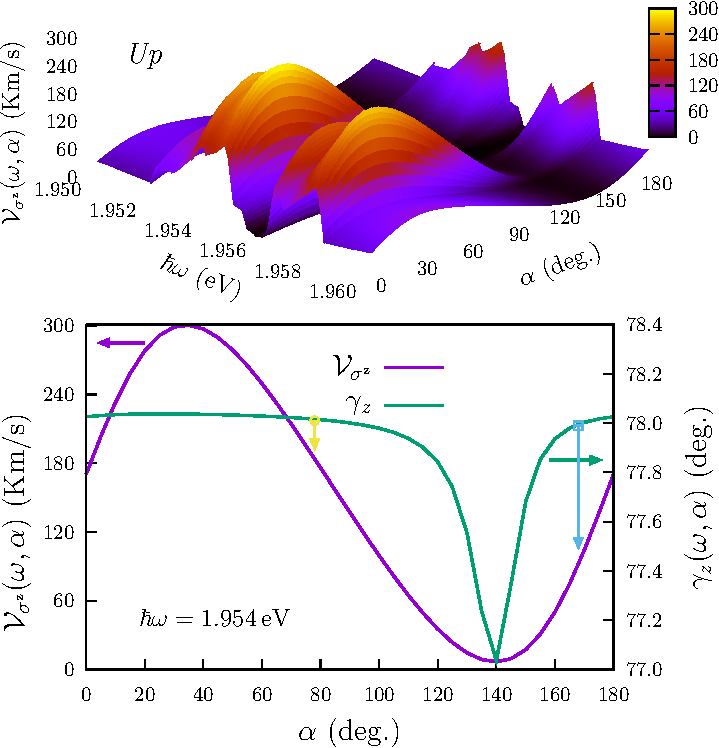
\includegraphics[width=\tama]{upplots/up-vsz-w2}
\caption{For the Up structure, the top panel shows $\calv_{\gs^\rmz} (\go,\ga)$
vs. $\hbar\go$ and $\ga$, and the bottom panel shows $\gamma_{\gs^\rmz}
(\go,\ga)$ (right scale, red line), and $\calv_{\gs^\rmz} (\go,\ga)$ (left
scale, black line), vs. $\ga$, for $\hbar\go=1.954$\,eV, i.e. along the
highest ridge shown in the 3D plot. }
\label{fig:up-vsz-w2}
\end{figure}

In this subsection, we calculate $\calv_{\gs^\rmz}(\omega,\alpha)$, Eq.
\eqref{eq:vs-mag}, for the case where the spin is fixed along $z$, i.e.
directed perpendicularly to the surface of the Up and Alt structures. Also, we
calculate $\gamma_{\gs^\rmz}(\go,\ga)$, Eq. \eqref{eq:gamma-ang}, which
determines the direction along which the injected electrons move along the
surface of  each structure. We mention that we have also made the analysis for
the cases when the spin  is directed along $\mathrm{x}$ or $\mathrm{y}$,
finding similar qualitative results to those presented below.
% 

\subsubsection{Up structure}\label{up:fs}

In the top panel of Fig. \ref{fig:up-vsz-w1}, we plot
$\mathcal{V}_{\sigma^{\mathrm{z}}} (\omega,\alpha)$ vs.
0.080\,eV$\leq\hbar\go\leq$0.096\,eV (similar energy range for the Up
structure shown in the left panel of Fig.~\ref{fig:vab-str-comp}) and
$0^\circ\leq\ga\leq 180^\circ$.
% 
We see a broad peak that maximizes at $\ga=35^{\circ}$ and $\hbar\go=
0.084$\,eV, with a value of $\mathcal{V}_{\sigma^{\mathrm{z}}}(\go,\ga) =
739.7$\,Km/s, and that the variation of $\mathcal{V}_{\sigma^{\mathrm{z}}}
(\omega,\alpha)$ as a function of $\ga$, which comes from the interplay of the
$\bfgmu$ tensor components as multiplied by the  trigonometric functions of
Eq.~\eqref{eq:vab-aw}, gives a sizable set of values between 739.7\,Km/s and
165.4\,Km/s, for 0.084\,eV$\leq\hbar\go\leq$0.090\,eV. 
% 
In the bottom panel, we show $\mathcal{V}_{\sigma^{\mathrm{z}}}
(\omega,\alpha)$ vs. $\ga$ (left scale, black line), at $\hbar\go= 0.084$\,eV,
thus following the ridge shown in the 3D plot of the top panel. 
Also,
we plot the
corresponding velocity angle $\gamma_{\gs^\rmz}(\omega,\alpha)$
(right scale, red line),
where it is very interesting to see that $\gamma_{\gs^z}(\omega,\alpha)$ is centered
at 64.55$^\circ$ with a rather small deviation of only $\pm 0.03^\circ$,
for the whole range of $\ga$. This results means that for $\hbar\go=0.084$ eV
and for all values of $\ga$, the electrons, with the chosen spin pointing along
$z$, will move at an angle of $\gamma_{\gs^\rmz}(\omega,\alpha) \sim
64.5^{\circ}$ with respect to the $x$ direction, with the range of  high
speeds $\mathcal{V}_{\sigma^{\mathrm{z}}} (\omega,\alpha)$ shown in the figure.
% 
Also, from Eq. \eqref{eq:gamma-par} we find that
$\gamma^\parallel_{\gs^\mathrm{z}} (\omega,\alpha)=\ga = 64.56^\circ$, with
$\mathcal{V}_{\sigma^{\mathrm{z}}} (\omega,\alpha) = 631.1$\,Km/s (see green
arrow), and that from Eq. \eqref{eq:gamma-perp},
$\gamma^\perp_{\gs^\mathrm{z}}(\omega,\alpha)=\ga-90^\circ=64.50^\circ$,
gives $\ga=154.50^\circ$, with
$\mathcal{V}_{\sigma^{\mathrm{z}}}(\omega,\alpha) = 191.5$ Km/s (see blue
arrow); thus, at $\hbar\go=0.084$ eV, an incident field polarized at $\alpha
\sim 65.5^\circ$ or $\sim 154.5^\circ$, injects electrons with their spin
polarized along $z$, which move parallel or perpendicular to the incident
electric field,  with a speed of 631.14\,Km/s or 191.5\,Km/s, respectively.

Now, we analyze the results for the second energy range of the Up structure
shown in the top right panel of Fig.~\ref{fig:vab-str-comp}. In the top panel
of Fig. \ref{fig:up-vsz-w2}, we plot $\mathcal{V}_{\sigma^{\mathrm{z}}}
(\omega,\alpha)$ vs. 1.950\,eV$\leq\hbar\go\leq$1.960\,eV and
$0^\circ\leq\ga\leq 180^\circ$.
% 
We see two broad peaks that maximize at $\ga=35^{\circ}$ and $\hbar\go=
1.954$\,eV, with a value of $\mathcal{V}_{\sigma^{\mathrm{z}}}(\go,\ga) =
193.5$\,Km/s, and at $\ga=35^{\circ}$ and $\hbar\go= 1.957$\,eV, with a value
of $\mathcal{V}_{\sigma^{\mathrm{z}}}(\go,\ga) = 170.6$\,Km/s. 
% 
We only analyze the highest  maximum in the bottom panel, where we  show
$\mathcal{V}_{\sigma^{\mathrm{z}}} (\omega,\alpha)$ vs. $\ga$ (left scale,
black line), at $\hbar\go= 1.954$\,eV, thus following the highest ridge shown
in the 3D plot of the top panel. Also, we plot the corresponding
velocity angle $\gamma_{\gs^\rmz}(\omega,\alpha)$ (right scale, red
line),
where in
this case we see that the values of $\gamma_{\gs^z}(\omega,\alpha)$ have more
dispersion, as a function of $\ga$, than for the lower energy range shown in
the bottom panel of Fig.~\ref{fig:up-vsz-w1}.
% 
However, $\gamma_{\gs^z}(\omega,\alpha)\sim 77.8^\circ$ is constant from
$\ga=0^\circ$ and up to $\ga\sim 85^\circ$. In this case, we find that
$\gamma^\parallel_{\gs^\mathrm{z}}(\omega,\alpha)=\ga=78.0^\circ$, with
$\mathcal{V}_{\sigma^{\mathrm{z}}}(\omega,\alpha) = 115.0$\,Km/s (see green
arrow), and that from Eq. \eqref{eq:gamma-perp},
$\gamma^\perp_{\gs^\mathrm{z}}(\omega,\alpha)=\ga-90^\circ=167.8^\circ$, gives
$\ga=77.8^\circ$, with $\mathcal{V}_{\sigma^{\mathrm{z}}}(\omega,\alpha) =
65.6$\,Km/s (see blue arrow). 
% 
Thus, through the correct choice of $\hbar\go$ and $\alpha$ we could inject
electrons, in this case with their spin polarized along $z$, which move parallel
or perpendicular to the incident electric field, with finite speeds.

% the maxima for
% $\hbar\go=0.084$ eV and $\alpha=35^{\circ}$, with
% $\mathcal{V}_{\sigma^{\mathrm{x}}}(\omega,\alpha)=219.6$ Km/s and
% $\mathcal{V}_{\sigma^{\mathrm{y}}}(\omega,\alpha)=280.3$ Km/s,
% $\gamma_{\mathrm{x}}(\omega,\alpha) = 79.3^{\circ}$, and 
% $\gamma_{\mathrm{y}}(\omega,\alpha) = 78.2^{\circ}$.

\begin{figure}[tb]
\centering
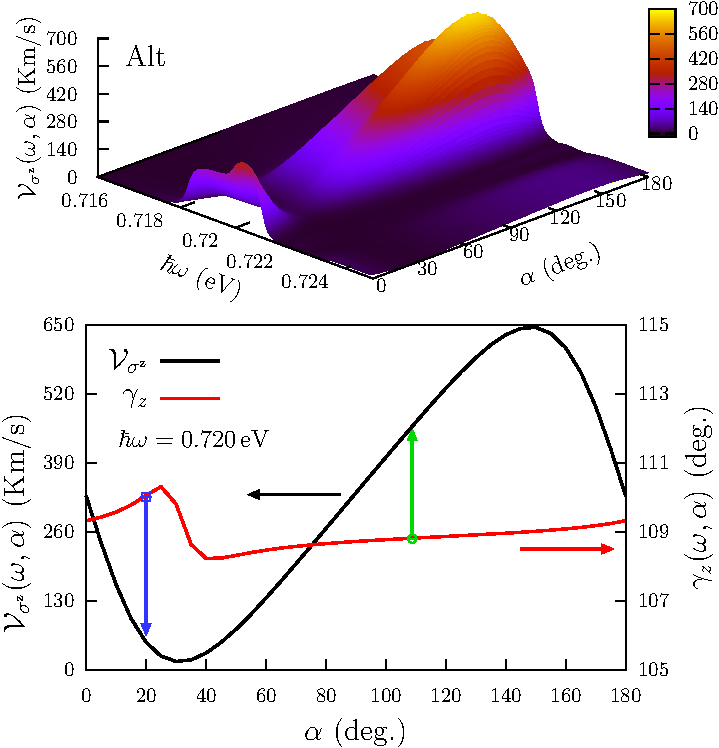
\includegraphics[width=\tama]{altplots/alt-vsz}
\caption{For the Alt structure, the top panel shows $\calv_{\gs^\rmz}
(\go,\ga)$ vs. $\hbar\go$ and $\ga$, and the bottom panel shows
$\gamma_{\gs^\rmz} (\go,\ga)$ (right scale, red line), and $\calv_{\gs^\rmz}
(\go,\ga)$ (left scale, black line), vs. $\ga$, for $\hbar\go=0.720$\,eV, i.e.
along the ridge shown in the 3D plot.}
\label{fig:alt-vsz}
\end{figure}

\subsubsection{Alt structure}

We proceed to analyze the Alt structure, just as we did with the Up structure, but
in this case, we only choose the lower energy range shown in the left central
panel of Fig.~\ref{fig:vab-str-comp}. 
% 
In the top panel of Fig. \ref{fig:alt-vsz}, we plot
$\mathcal{V}_{\sigma^{\mathrm{z}}} (\omega,\alpha)$ vs.
0.715\,eV$\leq\hbar\go\leq$0.725\,eV and $0^\circ\leq\ga\leq 180^\circ$. We
see a broad peak that maximizes at $\ga=150^{\circ}$ and $\hbar\go=
0.720$\,eV, with a value of $\mathcal{V}_{\sigma^{\mathrm{z}}}(\go,\ga) =
644.9$\,Km/s.
% 
In the bottom panel, we  show $\mathcal{V}_{\sigma^{\mathrm{z}}}
(\omega,\alpha)$ vs. $\ga$ (left scale, black line), at $\hbar\go= 0.720$\,eV,
 thus following the highest ridge shown in the 3D plot of the top
panel. Also, we plot the corresponding velocity angle $\gamma_{\gs^\rmz}
(\omega,\alpha)$ (right scale, red line), where now we see that
$\gamma_{\gs^z}(\omega,\alpha)$ is centered at $109.2^{\circ}$ having
variations of $\pm 1.0^{\circ}$ for $0^{\circ} \leq
\alpha \leq 180^{\circ}$.
% 
In this case, we find that $\gamma^\parallel_{\gs^\mathrm{z}} (\omega,\alpha) =
\ga = 108.8^\circ$, with $\mathcal{V}_{\sigma^{\mathrm{z}}} (\omega,\alpha) =
450.05$\,Km/s (see green arrow), and that from Eq. \eqref{eq:gamma-perp},
$\gamma^\perp_{\gs^\mathrm{z}}(\omega,\alpha)=\ga-90^\circ=110.0^\circ$,
gives $\ga=20.0^\circ$, with $\mathcal{V}_{\sigma^{\mathrm{z}}}
(\omega,\alpha) = 60.84$\,Km/s (see blue arrow). Thus, as for the Up structure,
we could inject electrons with a fixed spin which move parallel or perpendicular
to the incident electric field.

% Again, for the cases in which the spin polarization is parallel to the
% surface the maximum values are
% $\mathcal{V}_{\sigma^{\mathrm{x}}}(\omega,\alpha) = 297.8$ Km/s and
% $\mathcal{V}_{\sigma^{\mathrm{y}}}(\omega,\alpha) = 606.4$ Km/s,
% corresponding to $\gamma_{\mathrm{x}}(\omega,\alpha) = 116.3^{\circ}$
% $\gamma_{\mathrm{y}}(\omega,\alpha) = 110.1^{\circ}$ and both for
% $\alpha=150^{\circ}$, where the plots are not presented.

\subsection{Fixing velocity} 
\label{sec:res-fixvel}

We calculated $\mathcal{V}_{\mathrm{a}}(\omega,\alpha)$ (Eq. \eqref{eq:vv-mag})
fixing the electron velocity direction, $\rma$, to the $x$ or $y$ direction
along the surface of the Up and Alt structures. From Eqns. \eqref{eq:polar-ang}
and \eqref{eq:azimuthal-ang}, we determined the polar, $\theta_{\mathrm{a}}
(\omega,\alpha)$, and azimuthal, $\varphi_{\mathrm{a}} (\omega,\alpha)$, angles
corresponding to the direction of the spin.

\subsubsection{Up structure}

\begin{figure}[t]
\centering
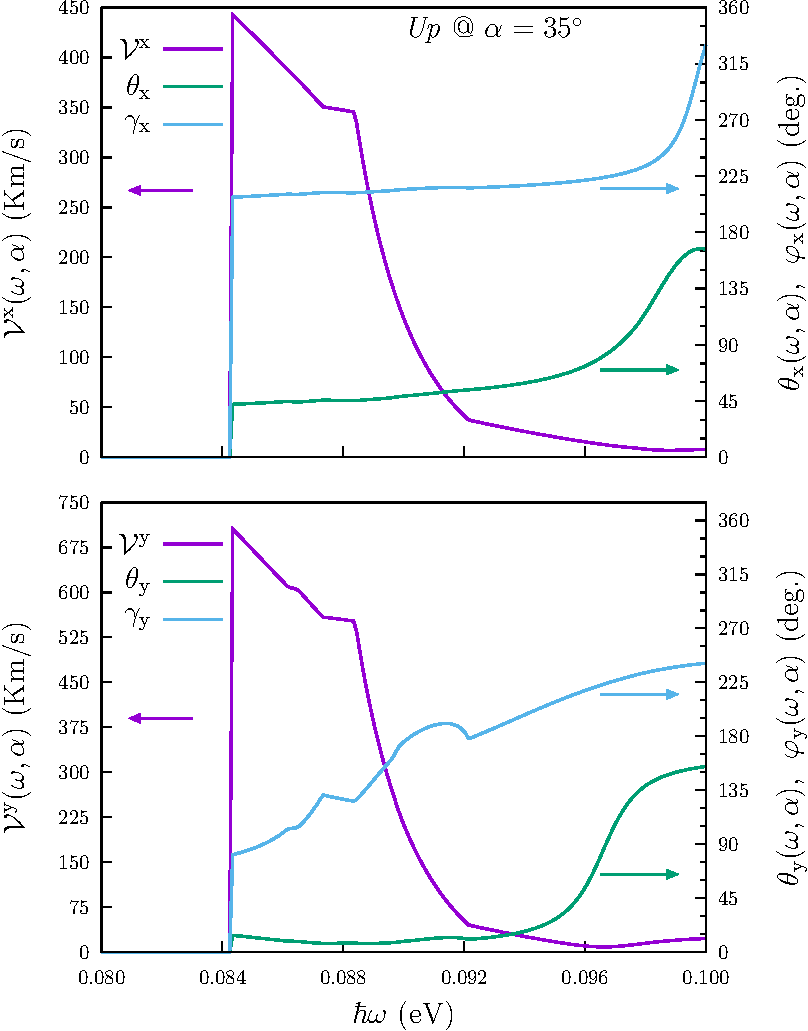
\includegraphics[width=\tama]{upplots/up-vx-vy-w1}
\caption{For the Up structure, we show
$\mathcal{V}_{\mathrm{a}} (\omega,\alpha)$
(left scale, black line),  
$\theta_{\mathrm{a}} (\omega,\alpha)$
(right scale, red line), and
$\varphi_{\mathrm{a}} (\omega,\alpha)$,
(right scale, blue line),
vs. $\hbar\go$, for $\ga=35^\circ$, 
and $\rma=x,y$.
}
\label{fig:up-vab-comp-rtp-1}
\end{figure}

For the Up structure, we find once again that  $\ga=35^{\circ}$ maximizes the
response. In Fig. \ref{fig:up-vab-comp-rtp-1}, we plot $\mathcal{V}_{\mathrm{a}}
(\omega,\alpha)$ (left scale, black line), $\theta_{\mathrm{a}}
(\omega,\alpha)$ (right scale, red line), and $\varphi_{\mathrm{a}}
(\omega,\alpha)$, (right scale, blue line), vs. $\hbar\go$, for $\rma=x,y$. 
% 
We see that for $\hbar\go=0.084$\,eV, the response has a maximum of
$\mathcal{V}_{\mathrm{x}} (\omega,\alpha)=431.7$\,Km/s, with
$\theta_{\mathrm{x}}(\omega,\alpha) = 42.5^{\circ}$, and
$\varphi_{\mathrm{x}}(\omega,\alpha) = 208.3^{\circ}$, and
$\mathcal{V}_{\mathrm{y}} (\omega,\alpha)=687.9$\,Km/s, with
$\theta_{\mathrm{y}}(\omega,\alpha) = 13.9^{\circ}$, and
$\varphi_{\mathrm{y}} (\omega,\alpha) = 82.1^{\circ}$. This means that the
spin is directed upward the third Cartesian quadrant of the $xy$ plane when the
electron moves along $x$, and is directed almost parallel to the $xy$ plane in
the first quadrant when it moves along $y$. 
% 
Also, from this figure we have that when the electron moves along $x$, the spin
direction is almost constant for all the energies across the peak of the
response, having
$42.5^{\circ}<\theta_{\mathrm{x}}(\omega,\alpha)<53.7^{\circ}$ and
$208.3^{\circ}<\varphi_{\mathrm{x}}(\omega,\alpha)<215.7^{\circ}$, and when
the electron moves along $y$, the spin polar angle has again small variations,
$11.3^{\circ}< \theta_{\mathrm{y}}(\omega,\alpha)<13.9^{\circ}$, but the
azimuthal angle has significant variations, $82.1^{\circ}<
\varphi_{\mathrm{y}}(\omega,\alpha)<182.4^{\circ}$.

\begin{figure}[t]
\centering
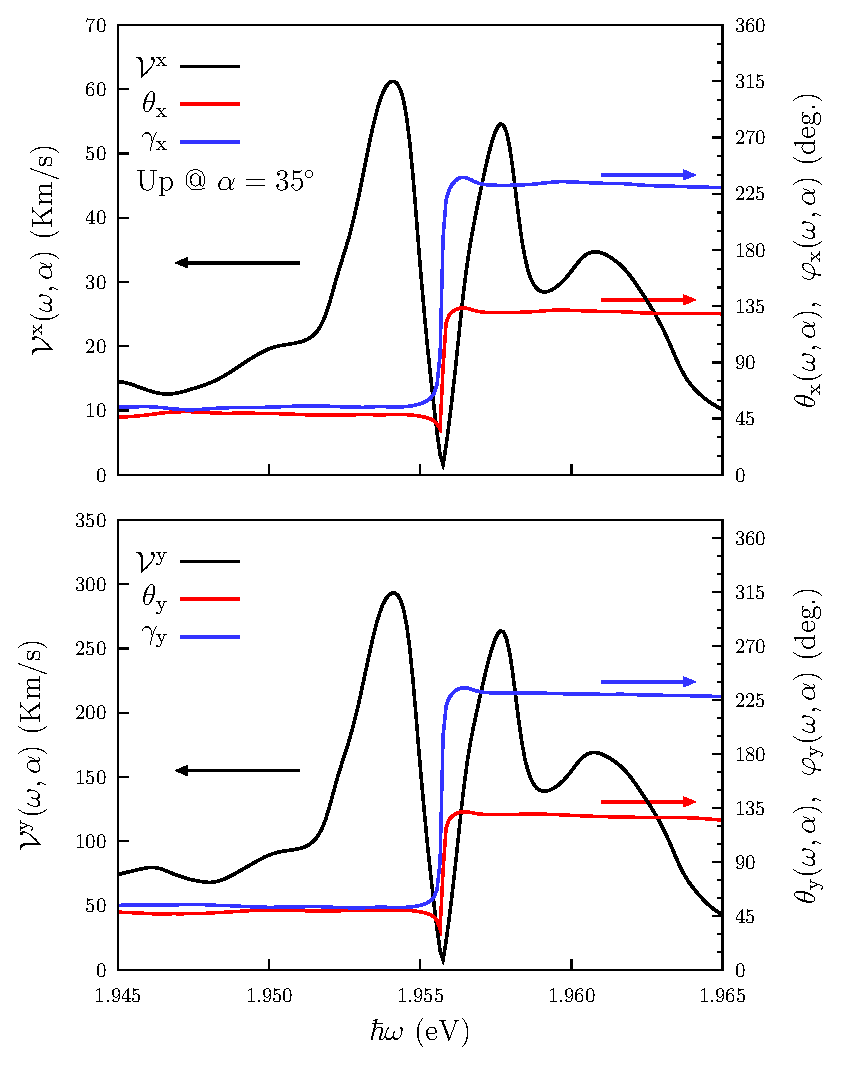
\includegraphics[width=\tama]{upplots/up-vx-vy-w2}
\caption{For the Up structure we show $\mathcal{V}_{\mathrm{a}}
(\omega,\alpha)$ (left scale, black line), $\theta_{\mathrm{a}}
(\omega,\alpha)$ (right scale, red line), and $\varphi_{\mathrm{a}}
(\omega,\alpha)$, (right scale, blue line), vs. $\hbar\go$, for
$\ga=35^\circ$, and $\rma=x,y$. }
\label{fig:up-vx-vy-w2}
\end{figure}
In Fig. \ref{fig:up-vx-vy-w2}, we plot $\mathcal{V}_{\mathrm{a}}
(\omega,\alpha)$ vs. $\hbar\go$, in the range where there are two local maxima
at $\hbar\go=1.954$\,eV and $\hbar\go=1.957$\,eV.
% 
The former is the largest of the two, with
$\mathcal{V}_{\mathrm{x}} (\omega,\alpha)=61.2$\,Km/s,
$\theta_{\mathrm{x}} (\omega,\alpha)=48.3^{\circ}$, and 
$\varphi_{\mathrm{x}} (\omega,\alpha)=54.3^{\circ}$,
for the electron moving along $x$, and
$\mathcal{V}_{\mathrm{y}} (\omega,\alpha)=293.2$\,Km/s,
$\theta_{\mathrm{y}} (\omega,\alpha)=49.8^{\circ}$, and 
$\varphi_{\mathrm{y}} (\omega,\alpha)=51.9^{\circ}$
for the electron moving along $y$.
% 
For the $\hbar\go=1.957$\,eV peak we obtain 
$\theta_{\mathrm{x}} (\omega,\alpha) = 129.8^{\circ}$, and 
$\varphi_{\mathrm{x}} (\omega,\alpha) = 231.7^{\circ}$, with 
$\mathcal{V}^{\mathrm{x}} (\omega,\alpha) = 54.6$\,Km/s, and
$\theta_{\mathrm{y}}(\omega,\alpha) =129.3$, and
$\varphi_{\mathrm{y}}(\omega,\alpha) = 230.7$, with 
$\mathcal{V}^{\mathrm{y}} (\omega,\alpha) = 263.7$\,Km/s. 
Checar que esto sea correcto para ambos maximos!!
We remark that these angles are almost
constant for all the energy values across the peak of these two local maxima, for
which the spin is directed upward in the first Cartesian quadrant of the $xy$
plane when it moves along either $x$ or $y$ directions. 

\subsubsection{Alt structure}

\begin{figure}[tb]
\centering
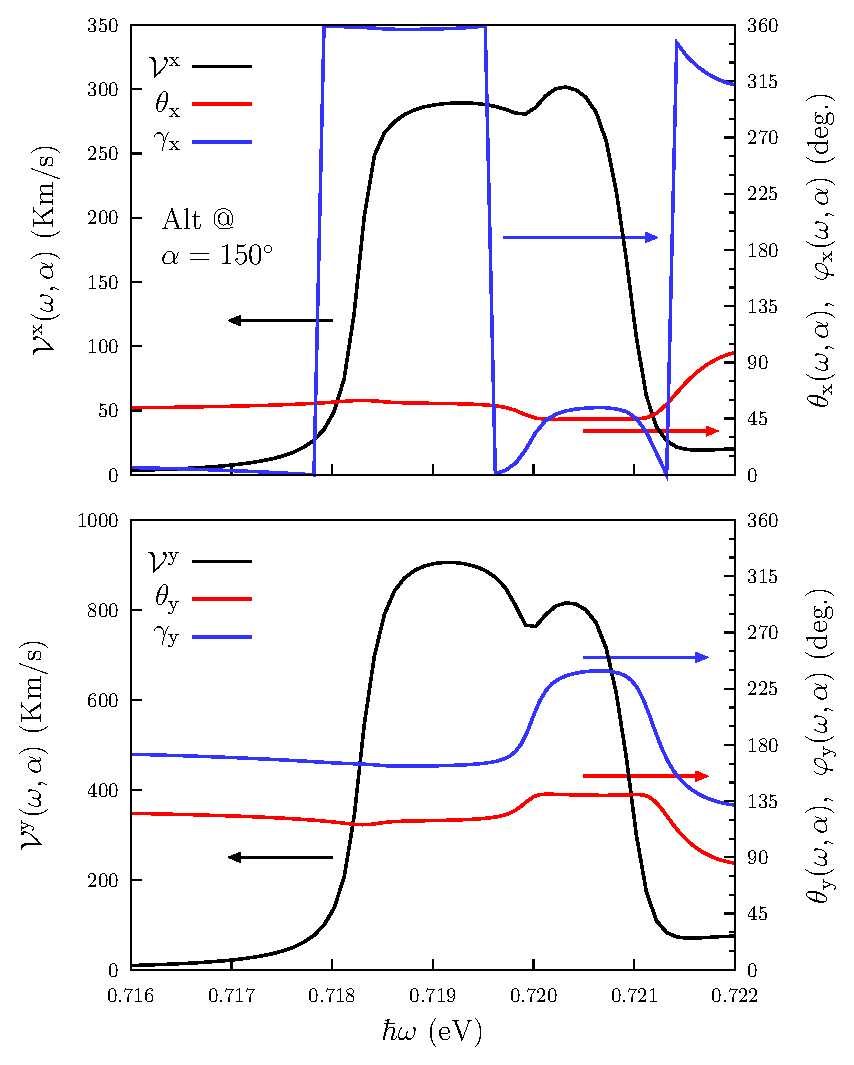
\includegraphics[width=\tama]{altplots/alt-vx-vy-w1}
\caption{For the Alt structure we show
$\mathcal{V}_{\mathrm{a}} (\omega,\alpha)$ (left scale, black line),
$\theta_{\mathrm{a}} (\omega,\alpha)$ (right scale, red line), and
$\varphi_{\mathrm{a}} (\omega,\alpha)$, (right scale, blue line), vs.
$\hbar\go$, for $\ga=150^\circ$, and $\rma=x,y$. }
\label{fig:alt-vx-vy-w1}
\end{figure}

\begin{figure}[tb]
\centering
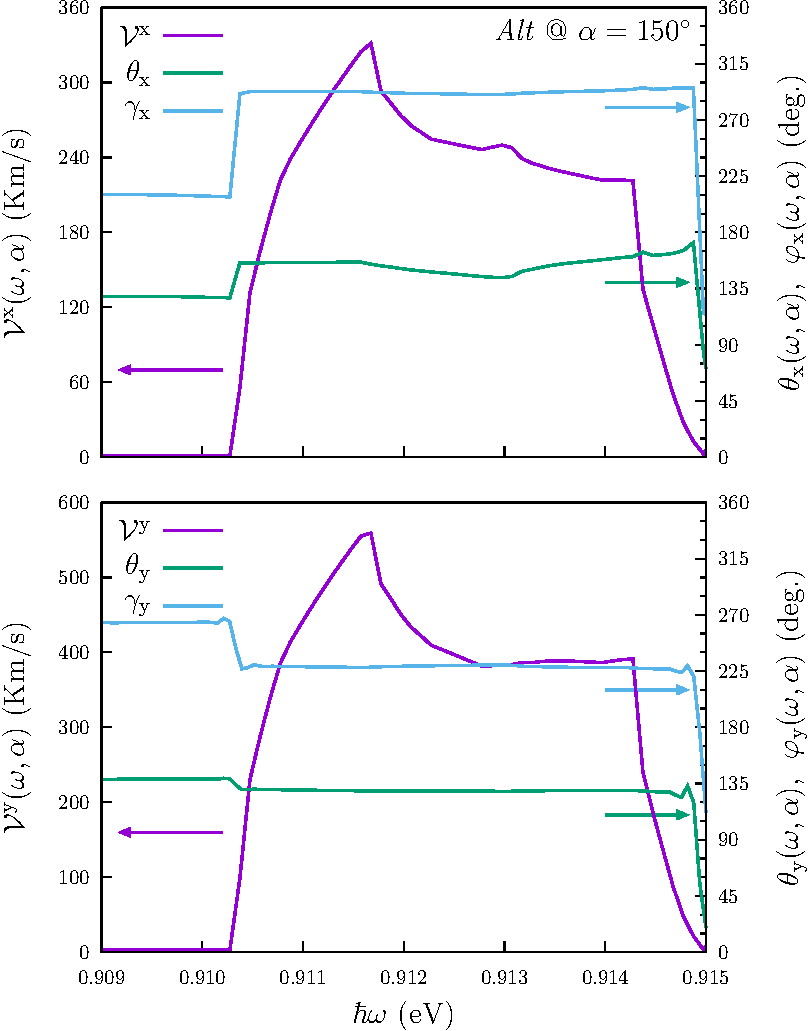
\includegraphics[width=\tama]{altplots/alt-vx-vy-w2}
\caption{For the Alt structure we show $\mathcal{V}_{\mathrm{a}}
(\omega,\alpha)$ (left scale, black line), $\theta_{\mathrm{a}}
(\omega,\alpha)$ (right scale, red line), and $\varphi_{\mathrm{a}}
(\omega,\alpha)$, (right scale, blue line), vs. $\hbar\go$, for
$\ga=150^\circ$, and $\rma=x,y$. }
\label{fig:alt-vx-vy-w2}
\end{figure}

In Figs. \ref{fig:alt-vx-vy-w1} and \ref{fig:alt-vx-vy-w2} we plot
$\mathcal{V}_{\mathrm{a}} (\omega,\alpha)$ (left scale, black line),
$\theta_{\mathrm{a}} (\omega,\alpha)$ (right scale, red line), and
$\varphi_{\mathrm{a}} (\omega,\alpha)$, (right scale, blue line), vs.
$\hbar\go$ in two different ranges, and  for $\rma=x,y$. In this case,
$\ga=150^\circ$,  maximizes both $\mathcal{V}_{\mathrm{x}} (\omega,\alpha)$,
and $\mathcal{V}_{\mathrm{y}} (\omega,\alpha)$, as a function of $\ga$.
% 
In Fig. \ref{fig:alt-vx-vy-w1} the absolute maxima is at
$\hbar\go=0.720$\,eV, with $\mathcal{V}_{\mathrm{x}}
(\omega,\alpha) = 301.7$\,Km/s, $\theta_{\mathrm{x}} (\omega,\alpha) =
44.5^{\circ}$, and $\varphi_{\mathrm{x}}(\omega,\alpha) = 51.2^{\circ}$,
and $\mathcal{V}_{\mathrm{y}} (\omega,\alpha) = 905.6$\,Km/s, with
$\theta_{\mathrm{y}} (\omega,\alpha) = 119.7^{\circ}$, and
$\varphi_{\mathrm{y}}(\omega,\alpha) = 163.4^{\circ}$. 
% 
Thus, the spin is directed upward the forth Cartesian quadrant of the $xy$
plane when the spin velocity is directed along $x$, and directed downward the
second Cartesian quadrant when the spin velocity is directed along $y$.
% 
Finally, in  Fig. \ref{fig:alt-vx-vy-w1}, the absolute maxima is at
$\hbar\go=0.911$\,eV, with $\mathcal{V}_{\mathrm{x}} (\omega,\alpha) =
276.3$\,Km/s, $\theta_{\mathrm{x}} (\omega,\alpha) = 154.6^{\circ}$, and
$\varphi_{\mathrm{x}}(\omega,\alpha) = 292.3^{\circ}$, and
$\mathcal{V}_{\mathrm{y}} (\omega,\alpha) = 468.6$\,Km/s, with
$\theta_{\mathrm{y}} (\omega,\alpha) = 129.2^{\circ}$, and
$\varphi_{\mathrm{y}}(\omega,\alpha) = 228.3^{\circ}$, implying that the spin
is directed downward the forth Cartesian quadrant of the $xy$ plane when the
spin velocity is directed along $x$, and directed downward the third Cartesian
quadrant when the spin velocity is directed along $y$.

\section{Conclusions} % (fold)
\label{sec:conclusions}

We have performed an \emph{ab initio} calculation for the SVI by one-photon
absorption of linearly polarized light in the Up and Alt 2D
hydrogenated graphene structures that and we made the calculation for the case
when the spin is polarized in the $z$ direction or when the velocity is
directed along $x$ or $y$; this effect does not seem to have been reported
previously on this kind of structures. 
% 
This SVI is very sensitive to the symmetry characteristics of the structures
presenting an anisotropic behavior. We found that the Up structure has
the most intense response for the spin directed along $z$ resulting in 
% 
$\mathcal{V}_{\sigma^{\mathrm{z}}} (\omega,\alpha) = 668.0$\,Km/s and 
% 
for an energy of the incoming beam of 0.084\,eV. Also the Alt structure
has the most intense response when the spin moves along the $y$ direction
resulting in 
% 
$\mathcal{V}^{\mathrm{y}} (\omega,\alpha) = 905.6$\,Km/s
% 
for an energy of the incoming beam of 0.720\,eV.
% 
The speed values obtained in here, are of the same order of magnitude
as those of Ref.~\onlinecite{najmaiePRB03} in 
unbiased semiconductor quantum well structures.
The spin relaxation time in pure and doped graphene is long enough in the order
from nanoseconds to milliseconds. \cite{wojtaszekPRB13,ertlerPRB09} The,
according to our results both are excellent candidates for the development of
spintronics devices that require PSC due to the high spin velocity transport.

\section{Acknowledgment} % (fold)

This work has been supported by \emph{Consejo Nacional de Ciencia y
Tecnolog\'ia} (CONACyT), M\'exico, Grant No. 153930.
R.Z.P. thank CONACyT for scholarship support.
\bibliography{article.bib}

\end{document}
